\documentclass{beamer}
\usepackage{ctex, hyperref}
\usepackage[T1]{fontenc}
\usepackage{tikz}
\usetikzlibrary{positioning}
% other packages
\usepackage{latexsym,amsmath,xcolor,multicol,booktabs,calligra}
\usepackage{graphicx,pstricks,listings,stackengine}
\usepackage{caption, subfigure}

% xmu beamer
\usepackage[blue]{TongjiBeamer}

\author[Author]{陈前 辛小雨}
\title{diversity is all your need}
\institute{同济大学}
\date{\today}


% defs6
\def\cmd#1{\texttt{\color{red}\footnotesize $\backslash$#1}}
\def\env#1{\texttt{\color{blue}\footnotesize #1}}

\lstset{
    basicstyle=\ttfamily\small,
    keywordstyle=\bfseries\color{red!0!green!0!blue!100},
    emphstyle=\ttfamily\color{red!100!green!0!blue!0},    % Custom highlighting style
    stringstyle=\color{red!0!green!100!blue!0},
    numbers=left,
    numberstyle=\small\color{gray!50},
    rulesepcolor=\color{red!20!green!20!blue!20},
    frame=shadowbox
}


\begin{document}
\begin{frame}
    \titlepage
    \begin{figure}[htpb]
       \begin{center}
            
\includegraphics[width=0.2\linewidth]{pic/tongji_logo.png}
        \end{center}
    \end{figure}
\end{frame}

\begin{frame}
\tiny
     \begin{columns}[T] % 创建左右分栏

    %     % --- 左栏:问题与挑战 ---
         \begin{column}{0.5\textwidth}
            \begin{block}{传统强化学习的困境}
                \begin{itemize}
                    \item \textbf{强依赖外部奖励}
                    \item 奖励设计成本高昂
                    \item 限制自主性与通用性
                    \item[$\rightarrow$] \textit{更像是被动的任务执行者}
                \end{itemize}
            \end{block}

            \begin{alertblock}{核心问题}
                 我们能否让智能体在\textbf{没有任务指令}的情况下,像人类一样\textbf{自主学习}
            \end{alertblock}
        \end{column}
        \begin{column}{0.5\textwidth}
            \begin{block}{解决方案:无监督强化学习}
                \textbf{核心思想:} 先学习,后做事 (Learn First, Act Later)
                \begin{itemize}
                    \item 在无奖励环境中,自主发现一系列\textbf{通用、可复用的技能} (Skills)。
                \end{itemize}
            \end{block}

            \textbf{关键方法:技能发现}
                \begin{itemize}
                    \item \textbf{目标:} 多样性 (Diversity is All You Need)
                    \item \textbf{工具:} 信息论 (Information Theory)
                    \begin{itemize}
                        \tiny
                        \item 最大化 \textbf{互信息} $I(S; Z)$ $\rightarrow$ \textit{技能可区分}
                        \item 最大化 \textbf{熵} $H(A|S, Z)$ $\rightarrow$ \textit{探索最大化}
                    \end{itemize}
                \end{itemize}
            
            \textbf{研究聚焦}
                提出一种新的无监督技能发现框架,旨在提升技能的\textbf{多样性、实用性与组合性}

         \end{column}
    \end{columns}

\end{frame}

\begin{frame}{应用价值}

    \begin{itemize}
        \item \textbf{解决稀疏奖励环境下的探索问题}
        \vspace{0.5cm}

        \item \textbf{作为分层强化学习的“积木块” (Primitives)}
        \begin{itemize}
            \item \textbf{上层策略}:选择“技能”(如“向前走”、“开门”)。
            \item \textbf{下层技能}:执行具体的“动作”序列。
            \item \textit{效果:} 显著缩短长时序任务的有效决策步长。
        \end{itemize}
        \vspace{0.5cm}
        
        \item \textbf{降低对人类监督的依赖}
        \begin{itemize}
            \item 适用于\textbf{交互成本低,但奖励评估成本高}(如需人类反馈)的场景。
            \item 智能体先自由探索学会技能,再由人类少量标注哪个技能有用。
        \end{itemize}
        \vspace{0.5cm}
        
        \item \textbf{在未知环境中自主发现潜在任务}
        \begin{itemize}
            \item 无监督地涌现出多样化技能,揭示了智能体在该环境中“能做什么”。
        \end{itemize}
    \end{itemize}

\end{frame}

\begin{frame}
    \frametitle{本文主要贡献 }

    \begin{itemize}
        \item \textbf{提出了一种无监督技能发现方法 DIAYN}
        \begin{itemize}
            \item 无需任何外部奖励函数,即可学习到有意义的技能。
        \end{itemize}
        \vspace{0.3cm}
        
        \item \textbf{设计了一个简洁且有效的目标函数}
        \begin{itemize}
            \item 基于信息论,能够驱动智能体涌现出如行走、跳跃等多样的技能。
            \item 仅通过无监督预训练,即可直接解决一些基准测试任务。
        \end{itemize}
        \vspace{0.3cm}
        
        \item \textbf{探索了技能的下游应用方法}
        \begin{itemize}
            \item 详细阐述了如何将学习到的技能应用于分层强化学习和模仿学习。
            \item 展示了如何快速利用已发现的技能来解决新任务。
        \end{itemize}
    \end{itemize}

    \begin{figure}[htbp] 
        \centering 
        % 请确保图片路径正确
        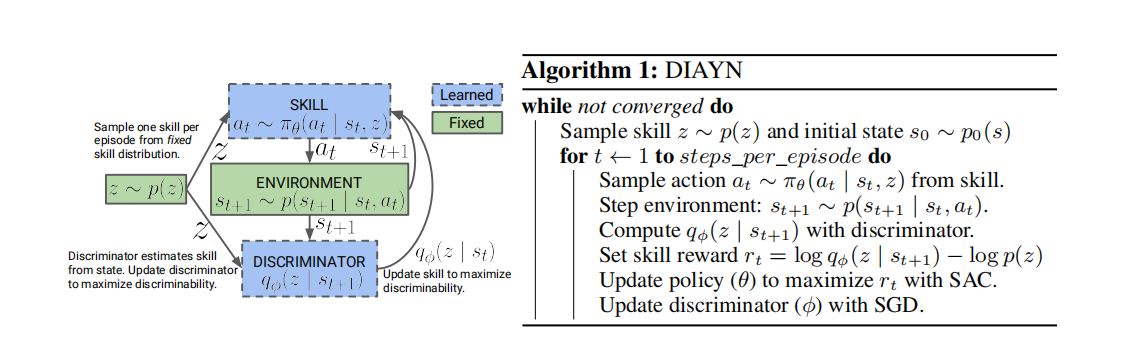
\includegraphics[width=0.75\textwidth]{pic/al1.png}
        \caption{DIAYN 算法框架示意图}
    \end{figure}

\end{frame}

\begin{frame}
    \tiny
    \frametitle{核心思想与实现方法}
    \begin{columns}[T]
        \begin{column}{0.6\textwidth}
            \begin{block}{核心思想 (Core Ideas)}
                \begin{enumerate}
                    \item \textbf{技能决定状态,使其可区分} \\
                    不同的技能 $z$ 应该引导智能体访问不同的状态 $s$。
                    \vspace{0.2cm}
                    
                    \item \textbf{鼓励探索,同时保持多样性} \\
                    每个技能的策略应尽可能随机(高熵),同时为保持可区分性,必须探索远离其他技能的状态空间。
                    \vspace{0.2cm}
                    
                    \item \textbf{通过状态而非动作来区分技能} \\
                    我们只关心技能产生的\textbf{结果}(状态变化),而不关心其\textbf{过程}(具体动作),因为某些动作可能不改变环境。
                \end{enumerate}
            \end{block}
        \end{column}

         \begin{column}{0.4\textwidth}
            \tiny
            \begin{block}{实现方法 (Approach)}
                \textbf{目标:} 最大化一个信息论驱动的目标函数
                \begin{itemize}
                    \item \textbf{最大化} 状态与技能的互信息 $I(S; Z)$ 
                     技能对状态有控制力,可区分
                    \vspace{0.2cm}
                    
                    \item \textbf{最大化} 条件动作熵 $H(A|S)$ 
                      策略行为尽可能随机,鼓励探索
                    \vspace{0.2cm}
                    
                    \item \textbf{最小化} 条件互信息 $I(A; Z | S)$ 
                     确保技能由状态而非动作区分
                \end{itemize}
            \end{block}
        \end{column}
    \end{columns}

    \begin{alertblock}{最终目标函数 (Objective Function)}
    \begin{align*}
        \mathcal{F}(\theta) 
        &\triangleq \underbrace{I(S; Z)}_{\text{可区分性}} 
                 + \underbrace{H[A \mid S]}_{\text{探索性}} 
                 - \underbrace{I(A; Z \mid S)}_{\text{解耦动作}} \\
        &= \underbrace{H[Z]}_{\text{技能多样}} 
           - \underbrace{H[Z \mid S]}_{\text{状态推断技能}} 
           + \underbrace{H[A \mid S, Z]}_{\text{技能内部探索}}
    \end{align*}
    \end{alertblock}

\end{frame}

\begin{frame}
    
    \frametitle{挑战与解决方案:变分推断 (Variational Inference)}
    \tiny
    \vspace{-0.2cm}
    \begin{columns}[T]
        % 左栏:挑战
        \begin{column}{0.5\textwidth}
            \begin{alertblock}{挑战:后验概率难以计算}
                目标函数中的互信息项 $I(S;Z)$ 依赖于条件熵 $H(Z|S)$,而计算它需要知道后验概率 $p(z|s)$。
                \vspace{0.3em}
                \begin{itemize}
                    \item $p(z|s) = \frac{p(s|z)p(z)}{p(s)}$
                    \item 其中分母 $p(s) = \int p(s|z)p(z)dz$ 需要对所有技能和轨迹积分,计算上是\textbf{不可行 (intractable)}的。
                \end{itemize}
            \end{alertblock}
        \end{column}

        % 右栏:解决方案
        \begin{column}{0.5\textwidth}
            \begin{block}{解决方案:引入鉴别器}
                我们引入一个可学习的分布 $q_\phi(z|s)$ 来\textbf{近似}真实的后验 $p(z|s)$。
                \vspace{0.3em}
                \begin{itemize}
                    \item $q_\phi(z|s)$ 是一个神经网络,通常称为\textbf{鉴别器 (Discriminator)} 或分类器。
                    \item \textbf{任务:} 输入状态 $s$,输出它由各个技能 $z$ 产生的概率。
                \end{itemize}
            \end{block}
        \end{column}
    \end{columns}

    % --- 下半部分:数学推导 ---
    \begin{block}{推导:变分下界 (Evidence Lower Bound, ELBO)}
        通过詹森不等式,我们可以推导出互信息 $I(S;Z)$ 的一个可计算的下界:
        \begin{align*}
            I(S; Z) &= \mathbb{E}_{p(s,z)}\left[\log \frac{p(z|s)}{p(z)}\right] \\
                    &= \mathbb{E}_{p(s,z)}\left[\log \frac{p(z|s)q_\phi(z|s)}{p(z)q_\phi(z|s)}\right] \\
                    &= \mathbb{E}_{p(s,z)}\left[\log \frac{q_\phi(z|s)}{p(z)}\right] + \mathbb{E}_{p(s)}\left[ D_{KL}(p(z|s) || q_\phi(z|s)) \right] \\
                    &\ge \mathbb{E}_{p(s,z)}\left[\log q_\phi(z|s)\right] + H(Z) \quad (\text{因为 } D_{KL} \ge 0)
        \end{align*}
        最终,我们将原始目标 $F(\theta)$ 替换为其下界 $G(\theta, \phi)$ 进行最大化。
    \end{block}

\end{frame}

\begin{frame}
     \frametitle{ 实现框架:Soft Actor-Critic (SAC)}

    \begin{alertblock}{选择 Soft Actor-Critic (SAC) 作为基础}
        \begin{itemize}
            \item \textbf{为何选择 SAC?} SAC 是一个基于\textbf{最大熵框架}的强大算法,其目标函数天生就包含策略熵 $H[a|s]$。
            
            \item \textbf{完美契合:} 这与 DIAYN 目标函数中的 $H[A|S,Z]$ 项(鼓励技能内部探索)完美对应。SAC 可以\textbf{自然地处理}这部分优化目标。
            
            \item \textbf{策略网络形式:} 学习到的策略以技能 $z$ 为条件,形式为:
            \[
                \pi_\theta(a | s, z)
            \]
            智能体根据当前状态 $s$ 和选定的技能 $z$ 来决定动作 $a$。
        \end{itemize}
    \end{alertblock}
\end{frame}

\begin{frame}
    \frametitle{核心机制:内在伪奖励 (Pseudo-Reward)}
    \framesubtitle{创造一个“虚拟”的奖励信号来引导学习}

    \begin{block}{问题:强化学习的“燃料”从何而来?}
        标准 RL 依赖于奖励。在无监督设定下,我们必须从 DIAYN 的目标函数中\textbf{“提取”}出一个内在奖励。
    \end{block}

    \begin{exampleblock}{伪奖励函数定义}
        我们将目标函数的一部分定义为每一步的奖励 $r_z(s, a)$:
        \[
            r_z(s, a) \triangleq \underbrace{\log q_\phi(z | s)}_{\text{主要驱动力}} - \underbrace{\log p(z)}_{\text{先验修正项}}
        \]
        
        \textbf{直观解释:}
        \begin{itemize}
            \item[$\bullet$] $\log q_\phi(z|s)$: 鉴别器 $q_\phi$ 认为当前状态 $s$ 多大程度上是由技能 $z$ 产生的。如果置信度高,说明状态 $s$ \textbf{很有“辨识度”},智能体就获得高奖励。
            \item[$\bullet$] $-\log p(z)$: 一个常数修正项(当 $p(z)$ 为均匀分布时),确保奖励在数学上与互信息严格对应。
        \end{itemize}
    \end{exampleblock}

    \begin{alertblock}{学习目标}
        智能体 (Agent) 的目标就是最大化这个累积的伪奖励,即学会\textbf{访问那些能让鉴别器轻松认出其技能的状态}。
    \end{alertblock}

\end{frame}

\begin{frame}{总结}
    \tiny
    \begin{columns}
    \begin{column}{0.5\textwidth}
    \begin{exampleblock}{ 整体学习流程}
            \begin{tikzpicture}[
                node distance=1cm,
                auto,
                block/.style={rectangle, draw, fill=blue!10, text width=6em, text centered, rounded corners, minimum height=3em},
                arrow/.style={thick,->,>=stealth}
            ]
                \node[block] (sample) {1. 采样技能 \\ $z \sim p(z)$};
                \node[block, below=of sample] (act) {2. 智能体执行 \\ $\pi_\theta(a|s,z)$};
                \node[block, below=of act] (reward) {3. 计算伪奖励 \\ $r_z(s,a)$};
                \node[block, below=of reward] (update) {4. 更新网络};
                
                \draw[arrow] (sample) -- (act);
                \draw[arrow] (act) -- (reward);
                \draw[arrow] (reward) -- (update);
                \draw[arrow] (update.west) to[out=180,in=180] node[left, text width=5em] {更新策略 $\pi_\theta$ (by SAC)} (act.west);
                \draw[arrow] (update.east) to[out=0,in=0] node[right, text width=6em] {更新鉴别器 $q_\phi$ (by Classifier Loss)} (reward.east);
            \end{tikzpicture}
            \end{exampleblock}
    \end{column}
    \begin{column}{0.5\textwidth}
    \begin{itemize}

    
    \item 技能 `z` 从一个固定的分类分布 $p(z)$ 中采样(通常是均匀的,比如有10个技能,每个被选中的概率是1/10)。
    \item 在每一轮(episode)游戏开始时,智能体先“想好”一个技能 `z`。
    \item 在整个这一轮中,智能体都使用这个固定的技能 `z` 来执行策略 $\pi_\theta(a|s,z)$。
    \item 智能体(Actor-Critic)的目标是最大化累积的伪奖励 $r_z(s, a)$。也就是说,它会努力去访问那些能让鉴别器 $q_\phi$ 轻松认出当前技能 `z` 的状态。
    \item 与此同时,鉴别器 $q_\phi$ 也在学习。它的目标是进行标准的监督学习分类任务:给定一大堆 `(状态, 技能)` 对,它要学会正确地从状态 `s` 预测出技能 `z`。
    
    \end{itemize}
    \end{column}
    \end{columns}
\end{frame}

\end{document} 